%% draft+final=finaldraft (no todos, but draft note at foot of page)
\documentclass[%
    draft, % comment draft to remove draft imprint at page foot
    %final, % give final when done. Overwrites draft. Removes todos.
    11pt,
    a4paper,
    fleqn,
    %openany %%chapter on right and left pages (no cleardoublepage)
]
{memoir}

%% Prevents figure and table placements in random locations.
\usepackage{float}

%% define control flags
\usepackage{ifthen}
\newboolean{printVersion}

\setboolean{printVersion}{false} % do not use colored links for print



\usepackage{lipsum}

%%%%%%%%%%%%%%%%%%%%%%%%%%
%% TOC space settings
%%%%%%%%%%%%%%%%%%%%%%%%%%
\setpnumwidth{3em}
\setrmarg{4em}


%%%%%%%%%%%%%%%%%%%%%%%%%%
%% floating environments
%%%%%%%%%%%%%%%%%%%%%%%%%%
\usepackage[final]          %w/o option final: no images in document-draft-mode
             {graphics}		% einbinden von graphiken

%\usepackage{caption}  %% not needed with documentclass memoir
\usepackage{subcaption} % neue subfigure-Umgebung %% should probably not be used with memoir: generates warning

%\usepackage[section]{placeins} %% \FloatBarrier

%% setup caption style (\usepackage{caption} w/o documentclass memoir)
\captionsetup[figure]{  labelfont       = {bf,color=captionCatergoryColor},
                        textfont        = {it,color=captionTextColor},
                        justification   = raggedright,
                        singlelinecheck = false,
                        position        = bottom,
                        format=hang
                        }
\captionsetup[table]{   labelfont       = {bf,color=captionCatergoryColor},
                        textfont        = {it,color=captionTextColor},
                        justification   = raggedright,
                        singlelinecheck = false,
                        position        = top,
                        format          = hang
                        }
%\captionsetup[table]{skip=7pt} %% mehr platz zwischen tabelle und caption

% move Text to Image. 1ex ~1 line of Text
% unfortunately: also valid for subcaptions.
%\setlength{\belowcaptionskip}{0ex}

% define how much text shall be on same page with large images
%% standard seems to be 0.20 --> 20%
%\renewcommand{\textfraction}{0.01}


%% Durchgängige Nummerierung von Figures und Tables:
%\usepackage{chngcntr}
%\counterwithout{figure}{chapter}
%\counterwithout{table}{chapter}


%define common figure sizes for subfigures
% -> redefined in each environment
\newlength{\subfigureWidth}
\setlength{\subfigureWidth}{0.22\textwidth}
\newlength{\graphicsHeight}
\setlength{\graphicsHeight}{25mm}

%% for page delte (see title-page-tex-file)
%\usepackage{atbegshi}

%%%%%%%%%%%%%%%%%%%%%%%%%%
%% table environments
%%%%%%%%%%%%%%%%%%%%%%%%%%
\usepackage{tabularx}
\newcolumntype{L}[1]{>{\raggedright\arraybackslash}p{#1}} % linksbündig mit Breitenangabe
\newcolumntype{C}[1]{>{\centering\arraybackslash}p{#1}} % zentriert mit Breitenangabe
\newcolumntype{R}[1]{>{\raggedleft\arraybackslash}p{#1}} % rechtsbündig mit Breitenangabe


%% allow multi-row
\usepackage{multirow}
\usepackage{booktabs} %% toprule, midrule and bottomrule for tables



%%%%%%%%%%%%%%%%%%%%%%%%%%
%%for color definitions
%%%%%%%%%%%%%%%%%%%%%%%%%%
\usepackage{xcolor}
%%------------------
%% new colors

% defines the main color theme
% command \colorlet is used to derivate colors from this main color
\definecolor{thesisMainColor}{rgb}{0.36, 0.54, 0.66} %% (92,138,167)@256=100%   #5C8AA7
\definecolor{thesisSecondaryColor}{rgb}{1.00,0.60,0.10} % {cmyk}{0.1, 0.6, 1, 0} %% (255,154,26)@256=100   #FF9A1A

\colorlet{thesisMainColor_dark5}{black!5!thesisMainColor}
\colorlet{thesisMainColor_dark10}{black!10!thesisMainColor}
\colorlet{thesisMainColor_dark15}{black!15!thesisMainColor}
\colorlet{thesisMainColor_dark20}{black!20!thesisMainColor}

% DFKI colors
\definecolor{dfki1}{cmyk}{0.9, 0.55, 0.1, 0}	% DFKI blue
\definecolor{dfki2}{cmyk}{0.1, 0.6, 1, 0}		% DFKI orange
\definecolor{dfki3}{cmyk}{0, 0.89, 0.06, 0.1}	% Magenta Coler Tetrad
\definecolor{dfki4}{cmyk}{0.89, 0, 0.83, 0.1}	% Green Coler Tetrad

\definecolor{grey80}{gray}{0.2}
\definecolor{grey60}{gray}{0.4}
\definecolor{grey40}{gray}{0.6}
\definecolor{grey20}{gray}{0.8}
\definecolor{grey10}{gray}{0.9}



%%------------------
%% derived colors


%chapter numbers
\colorlet{chaptercolor}{thesisMainColor_dark5}

%tables
\colorlet{tableheadingcolor}{thesisMainColor!40}
\colorlet{tablesubheadingcolor}{thesisSecondaryColor!30}

%captions
\colorlet{captionCatergoryColor}{thesisMainColor_dark20}%{grey80!60!thesisMainColor}
\colorlet{captionTextColor}{captionCatergoryColor}%{grey60!60!thesisMainColor}

%itemize
\colorlet{itemicolor}{thesisMainColor_dark5}
\colorlet{itemiicolor}{itemicolor}
\colorlet{itemiiicolor}{itemicolor}

%description text
\colorlet{descriptionColor}{captionCatergoryColor}%{black!20!thesisMainColor}%{thesisMainColor!70!black}%

%footnotes
\colorlet{footnoteMarkColor}{captionCatergoryColor}
\colorlet{footnoteRuleColor}{footnoteMarkColor}
%\colorlet{footnoteTextColor}{footnoteMarkColor} %%not yet needed, color is given by ruleColor


%hyperrefcolors
% we need this switch because of the \refFig etc definitions
\ifthenelse{\boolean{printVersion}}
{%if true
    \colorlet{thesisLinkColor}{black}
    \colorlet{thesisUrlColor}{black}
    \colorlet{thesisCiteColor}{black}
}
{%else
    \colorlet{thesisLinkColor}{captionCatergoryColor}%{black}%{thesisMainColor}%{blue!60!black}
    \colorlet{thesisUrlColor}{thesisMainColor}%{blue!60!black}
    \colorlet{thesisCiteColor}{thesisMainColor}%{thesisSecondaryColor}%{green!60!black}
}


%colors in for acronyms
\colorlet{acroextraColor}{thesisLinkColor}

%color for chapter quotes
\colorlet{quoteColor}{chaptercolor!70!grey80}%{captionTextColor}%

% colors for structure graphs
%% colors for all graph types
\colorlet{structureGraphBgColorMain}{white}%{thesisSecondaryColor!5}%
\colorlet{structureGraphFrameColorMain}{black}%{thesisSecondaryColor!30}%
\colorlet{structureGraphBgColorTitleMain}{grey60}%{thesisSecondaryColor!30}%
\colorlet{structureGraphTextTitleColorMain}{thesisSecondaryColor!80}%{black!50!white}%
\colorlet{structureGraphTextTitleColorBigtopicbox}{white}
%\colorlet{structureGraphContentColor}{thesisMainColor!75} %%not needed, take title_bg_color

%% topic graph
\colorlet{structureGraphBackgroundColorBigtopicbox}{grey20}%{thesisSecondaryColor!5}%
\colorlet{structureGraphFrameColorBigtopicbox}{thesisSecondaryColor!30}%{black!55!white}%
\colorlet{structureGraphTitleBackgroundColorBigtopicbox}{grey40}%{thesisSecondaryColor!45}%

\colorlet{structureGraphBackgroundColorTopicbox}{thesisMainColor!5}
\colorlet{structureGraphFrameColorTopicbox}{thesisMainColor!50}%{thesisSecondaryColor!30}%
\colorlet{structureGraphTitleBackgroundColorTopicbox}{thesisMainColor_dark5}%{thesisMainColor!75}
\colorlet{structureGraphTextTitleColorTopicbox}{thesisMainColor!10}%{white}%{thesisSecondaryColor!30}%

%% chapter graph
\colorlet{structureGraphBackgroundColorChapterbox}{thesisMainColor!1}%{structureGraphBackgroundColorTopicbox}
\colorlet{structureGraphFrameColorChapterbox}{grey40}%{structureGraphFrameColorTopicbox}
\colorlet{structureGraphTitleBackgroundColorChapterbox}{thesisMainColor_dark5}%{structureGraphTitleBackgroundColorTopicbox}
\colorlet{structureGraphTextTitleColorChapterbox}{thesisMainColor!1}%{structureGraphTextTitleColorTopicbox}
 %%own colors with names




%print draft text indo background
\usepackage{rotating}
\usepackage{eso-pic}
%\usepackage{color}
\usepackage{type1cm}

\newcommand{\printdraft}[1][Draft]{
    \AddToShipoutPicture{%
       \AtPageCenter{%\section
         \makebox(0,0){%
           \rotatebox{50}{
               \textcolor[gray]{0.95}{
               		\fontsize{7cm}{7cm}%
               		\selectfont{#1}
                }
            }
          }
        }
    }
}

\usepackage[bookmarks,bookmarksopen=false,bookmarksnumbered=true,pdftex,pdfhighlight=/N,
  linkcolor=thesisLinkColor,%blue!60!black,
  urlcolor=thesisUrlColor,%blue!60!black,
  citecolor=thesisCiteColor,%green!60!black,
  colorlinks=true,
  pdftitle={},
  pdfsubject={},  % insert subtitle
  pdfkeywords={Wheeled-Leg Rover, Active Suspension System, Solar Array, Solar Tracking, SherpaTT, Sherpa},
  pdfauthor={Georges L. J. Labreche},
  %final %%use links also in draft mode
  ]{hyperref}


\usepackage{ifdraft} %\ifdraft, \ifoptiondraft, \ifoptionfinal

%% in final document for print: no colored links(?)
\ifdraftdoc
    \hypersetup{final}  %use hyper-final option in draft mode: standard-links
    %\printdraft	        % Print "Draft" Watermark
\else
    %\hypersetup{draft} % use hyper-draft in final document: no links
\fi



%% for faster use of pdflatex
%% DO NOT USE FOR PDF/A compability!
%%\pdfcompresslevel=5
%% check styles/pdf_a_compability.tex





%%%%%%%%%%%%%%%%%%%%%%%%%%
%% setup todo style
%%%%%%%%%%%%%%%%%%%%%%%%%%
%usage: \todo[inline]{blah}
%       \todo{blubb}
\usepackage[obeyFinal]{todonotes}              % todos in text
\presetkeys{todonotes}{fancyline,
                        backgroundcolor=thesisSecondaryColor!50,
                        bordercolor=thesisMainColor,
                        linecolor=thesisMainColor,
                        size=\scriptsize %\footnotesize
                       }{}
\tikzset{/tikz/notestyleraw/.append style={text=thesisMainColor}} % set textcolor
\setlength{\marginparwidth}{2.2cm} % Rand-Notizenbreite einstellen \todo{blahblubb}

\ifdraftdoc
    %%--- define a new todo-list style ---
    \makeatletter
    \def\myaddcontentsline#1#2#3{%
      \addtocontents{#1}{\protect\contentsline{#2}{#3}{\textcolor{thesisMainColor}{\thepage\ ~~ (\textbf{Chapter \thechapter})}}{}}}
    \renewcommand{\@todonotes@addElementToListOfTodos}{%
        \if@todonotes@colorinlistoftodos%
            \myaddcontentsline{tdo}{todo}{{%
                \colorbox{\@todonotes@currentbackgroundcolor}%
                    {\textcolor{\@todonotes@currentbackgroundcolor}{o}}%
                \ \@todonotes@caption}}%
        \else%
            \myaddcontentsline{tdo}{todo}{{\@todonotes@caption}}%
        \fi}%
    \newcommand*\mylistoftodos{%
      \begingroup
           \setbox\@tempboxa\hbox{Chapter 9.9 (p. 999)}%
           \renewcommand*\@tocrmarg{\the\wd\@tempboxa}%
           \renewcommand*\@pnumwidth{\the\wd\@tempboxa}%
           \textcolor{thesisMainColor}{%[rgb]{1.00,0.00,0.00}{
            %\pagecolor{thesisSecondaryColor!50}%
            \begin{small}
                \listoftodos%
            \end{small}
            \todototoc%
            }
        %\clearpage ~~
        %\afterpage{\nopagecolor}
        \clearpage

      \endgroup
    }
    \makeatother
\else
    \newcommand{\mylistoftodos}{}
\fi %end: ifdraftdoc



%%%%%%%%%%%%%%%%%%%%%%%%%%%%
%% page style setup FCordes
%%%%%%%%%%%%%%%%%%%%%%%%%%%%
% ********************************************************************
% composed by Florian Cordes @ DFKI RIC
%
% to be used with documentclass memoir:
% \documentclass[11pt,a4paper]{memoir}
%
% January 2018
% ********************************************************************

\NeedsTeXFormat{LaTeX2e}
\ProvidesPackage{phdDocumentStyle_FCordes}[2018/01/19 v1.0 Style for PhD document]



%Zeilenumbruch, falls overfull hbox
\sloppy
%\relax

%%%%%%%%%%%%%%%%%%%%%%%%%%%%%%%%%%%%%%%%%%%
%% define what happens when
%% draft option is set in documentclass
%%%%%%%%%%%%%%%%%%%%%%%%%%%%%%%%%%%%%%%%%%%
\newcommand{\myDraftNote}[0]{\color{thesisSecondaryColor}{\textit{Draft version: \today}}}
\newcommand{\myFinalDraftNote}[0]{\color{thesisSecondaryColor}{\textit{Final Draft (\today)}}}

\ifdraftdoc
    \makeevenfoot{plain}{}{\thepage}{\myDraftNote}
    \makeoddfoot{plain}{\myDraftNote}{\thepage}{}
    \makeevenfoot{ruled}{\thepage}{}{\myDraftNote}
    \makeoddfoot{ruled}{\myDraftNote}{}{\thepage}
\fi

\makeevenhead{ruled}{\scshape Chapter \leftmark}{}{}
\makeoddhead{ruled}{}{}{\itshape\rightmark}


%%%%%%%%%%%%%%%%
%% Itimisation
%%%%%%%%%%%%%%%%
\newlength{\sqsize}
\setlength{\sqsize}{0.8ex}
\newcommand*\sq{\raisebox{0.4\sqsize}{\rule{\sqsize}{\sqsize}}} % define a small square for itemize bullet

\renewcommand{\labelitemi}{${\color{itemicolor}\sq}$}%\blacksquare}$}
\renewcommand{\labelitemii}{${\color{itemiicolor}\blacktriangleright}$} %\bullet}$}
\renewcommand{\labelitemiii}{${\color{itemiiicolor}\square}$}




%%%%%%%%%%%%%%%%
%% Description
%%%%%%%%%%%%%%%%
\renewcommand*{\descriptionlabel}[1]{\hspace
                                     \labelsep
                                     \normalfont
                                     \textbf{\color{descriptionColor}{#1}}
                                 }




%%%%%%%%%%%%%%%%%%%
%% footnote formatting and colors
%%%%%%%%%%%%%%%%%%%
%change the mark (reference-number)
\renewcommand\thefootnote{\textcolor{footnoteMarkColor}{
                                            (\alph{footnote})%
                                            %\arabic{footnote})%
                                            }}

%change the text at the bottom of the page
\renewcommand{\foottextfont}{\footnotesize}%\color{footnoteTextColor}}

%change the rule above the footnote
\renewcommand*{\footnoterule}{%
    \kern-3pt%
    \color{footnoteRuleColor}\hrule width 0.4\columnwidth %%also sets the text-body color when written like this
    \kern 2.6pt
    }

\setlength{\footnotesep}{2ex}       % the separation between footnotes
\setlength{\footmarkwidth}{1.5em}   % indention of complete footnote textblock
\setlength{\footmarksep}{0.3em}       % indention of second and following lines
\setlength{\footparindent}{2em}     % indention of paragraph within footnote

%make a refernce-command for footnotes
\makeatletter
\newcommand\fnref[1]{\protected@xdef\@thefnmark{\ref{#1}}\@footnotemark}
\makeatother

%do not reset counter per chapter
\counterwithout*{footnote}{chapter}

% footnotes shall be at the bottom of the page, even wenn a figure has [b] option
\feetbelowfloat

%%%%%%%%%%%%%%%%%%%%%%%%%%%%%%
%% Define sectioning depth
%%%%%%%%%%%%%%%%%%%%%%%%%%%%%%
\setsecnumdepth{subsection}
\settocdepth{section}


%%%%%%%%%%%%%%%%%%%%%%%%%%%%%%
%% new line spacing
%%%%%%%%%%%%%%%%%%%%%%%%%%%%%%
\setSingleSpace{1.05}
\SingleSpacing





%%%%%%%%%%%%%%%%%%%%%%%%%%%%%%%%%%%%%%%%%%%
%% define the text field for the pages
%%%%%%%%%%%%%%%%%%%%%%%%%%%%%%%%%%%%%%%%%%%
\newlength{\myRegularParskip}
\setlength{\myRegularParskip}{1.8mm}

\newlength{\myCenterSpaceOffset}
\setlength{\myCenterSpaceOffset}{0.7mm} % pos increases spacing in center of double page

\textheight235mm              % Höhe des Textbereichs
\textwidth160mm             % Breite des Textbereichs
\topmargin-20mm
\topskip5mm
\headheight20mm
\headsep3mm
\setlength\evensidemargin{-\myCenterSpaceOffset} % pos vals to move in
\setlength\oddsidemargin{\myCenterSpaceOffset}   % neg vals to move in
\footskip15mm
\headwidth\textwidth

\setlength\parindent{0mm}
\setlength\parskip{\myRegularParskip}


%%%%%%%%%%%%%%%%%%%%%%%%%%%%%%
%% Defines for Chapter Style
%%%%%%%%%%%%%%%%%%%%%%%%%%%%%%
\usepackage{kpfonts}

\newcommand\numlifter[1]{\raisebox{-2.5cm}[0pt][0pt]{\smash{#1}}} % how low can you go?
\newcommand\numindent{\kern10pt} %space from right margin
\newlength\chaptertitleboxheight
\makechapterstyle{cordesDiss}{
  \renewcommand\printchaptername{\raggedleft}
  \renewcommand\printchapternum{%
    \begingroup%
    \leavevmode%
    \chapnumfont%
    \strut%
    \numlifter{\thechapter}%{\fontfamily{pnc}\selectfont \thechapter} }%
    \numindent%
\endgroup%
}
  \renewcommand*{\printchapternonum}{%
    \vphantom{\begingroup%
      \leavevmode%
      \chapnumfont%
      \numlifter{\vphantom{9}}%
      \numindent%
      \endgroup}
    \afterchapternum}
  \setlength\midchapskip{0pt}
  \setlength\beforechapskip{0.5\baselineskip}
  \setlength{\afterchapskip}{3\baselineskip}
  \renewcommand\chapnumfont{%
    \fontsize{4cm}{0cm}%
    \bfseries%
    \sffamily%
    \color{chaptercolor}%
  }
  \renewcommand\chaptitlefont{%
    \normalfont%
    \huge%
    \bfseries%
    \raggedleft%
  }%
  \settototalheight\chaptertitleboxheight{%
    \parbox{\textwidth}{\chaptitlefont \strut bg\\bg\strut}}
  \renewcommand\printchaptertitle[1]{%
    \parbox[t][\chaptertitleboxheight][t]{\textwidth}{%
      %\microtypesetup{protrusion=false}% add this if you use microtype
      \chaptitlefont\fontsize{0.9cm}{\baselineskip}\selectfont\strut ##1\strut}%FC
      %\chaptitlefont \strut ##1\strut}% ORIGINAL
      %\HUGE\bfseries\strut ##1\strut}% FC
}}

%% now set the style active
\chapterstyle{cordesDiss}
\aliaspagestyle{chapter}{plain} % just to save some space: no header

%\createplainmark{toc}{both}{\acronym}


%% -----------------------------
%% floating environment options
%% -----------------------------

% define how much text shall be on same page with large images
%% standard seems to be 0.20 --> 20%
%\renewcommand{\textfraction}{0.01}


%% setup caption style
\captionsetup[figure]{labelfont={bf,color=captionCatergoryColor},textfont={it,color=captionTextColor},justification=raggedright,singlelinecheck=false,format=hang}
\captionsetup[table]{labelfont={bf,color=captionCatergoryColor},textfont={it,color=captionTextColor},justification=raggedright,singlelinecheck=false,format=hang}
%\captionsetup[table]{skip=7pt} %% mehr platz zwischen tabelle und caption

%% Durchgängige Nummerierung von Figures und Tables:
%\usepackage{chngcntr}
%\counterwithout{figure}{chapter}
%\counterwithout{table}{chapter}



%% --------------------
%% special functions
%% --------------------

% acronym
\newcommand{\dissAcroextra}[1]{\acroextra{~\\[-0.6ex]\textcolor{acroextraColor}{\scriptsize{(#1)}}}}

% quote at beginning of chapter
\newcommand{\shinyChapterQuote}[2]{
\begin{quote}\hypersetup{hidelinks=true}
    \textcolor{quoteColor}{
        \emph{#1}
        \newline\indent\qquad -- #2
    }
\end{quote}
}

% a command to add (smaller) extra info in captions of Figures and Tables
\newcommand{\dissExtraCaption}[1]{\newline\footnotesize{#1}}

%% symbols
\newcommand{\dissCheck}{\textcolor{thesisMainColor}{$\mathbf{\checkmark}$}}
\newcommand{\dissUncheck}{\textcolor{thesisSecondaryColor}{$\mathbf{\times}$}}
\newcommand{\myTTAmark}{\textcolor{thesisSecondaryColor!80}{\ensuremath{^\star}}\xspace}%{\ensuremath{^\circledast}}\xspace}%{\ensuremath{^\blacklozenge}}\xspace}



%%%%%%%%%%%%%%%%%%%%%%%%%%
%% define the boxes for thesis structure graph
%%%%%%%%%%%%%%%%%%%%%%%%%%


%
% use as option in tcolorbox environment:
% [code={\pgfkeysalsofrom{\outerboxoptions}}, otheroption=...]
%
\def\outerboxoptions{ %the thesis frame
    colback=structureGraphBackgroundColorBigtopicbox,%grey10,%structureGraphBgColorMain,
    colframe=structureGraphFrameColorBigtopicbox,%structureGraphFrameColorMain,
    colbacktitle=structureGraphTitleBackgroundColorBigtopicbox,%structureGraphBgColorTitleMain,
    coltitle=thesisMainColor!50!black,%structureGraphTextTitleColorMain,
    left=1mm,
    right=1mm,
    boxrule=0.8pt
}

\def\topicboxoptions{
    %sidebyside,righthand width=.26\textwidth,
    colback=structureGraphBgColorMain,
    colframe=structureGraphFrameColorMain,
    colbacktitle=structureGraphBgColorTitleMain,
    coltitle=structureGraphTextTitleColorMain,
    boxrule=0.8pt,
    left=1mm,
    right=1mm
}


\def\chapterboxoptions{
    colback=structureGraphBackgroundColorChapterbox,
    colframe=structureGraphFrameColorChapterbox,
    colbacktitle=structureGraphTitleBackgroundColorChapterbox,
    coltitle=structureGraphTextTitleColorChapterbox,
    boxrule=0.6pt,
    left=0.6mm,
    right=0.6mm,
    top=1mm,
    bottom=1mm
    %drop large lifted shadow,
}

\def\outerrasteroptions{
    raster width=\linewidth,
    raster columns=1,
    %% Forces same height in all columns on same row
    raster equal height=rows,
    raster every box/.style={valign=center, halign=center}
}

\def\innerrastersinglecoloptions{
    raster columns=1,
    raster width=0.5\linewidth, %otherwise inherits from outer raster
    %% Forces same height in all columns on same row
    raster equal height=rows,
    raster every box/.style={valign=center, halign=center},
}

\def\innerrasterdualcoloptions{
    raster columns=2,
    raster width=0.992\linewidth, %otherwise inherits from outer raster
    %% Forces same height in all columns on same row
    raster equal height=rows,
    raster every box/.style={valign=center, halign=center},
}

\def\innerrastertriplecoloptions{
    raster columns=3,
    raster width=0.992\linewidth, %otherwise inherits from outer raster
    %% Forces same height in all columns on same row
    raster equal height=rows,
    raster every box/.style={valign=center, halign=center},
}









\newcommand{\drawChapterbox}[2]{
    %\begingroup
        \hypersetup{hidelinks=true}%
        \begin{tcolorbox}[code={\pgfkeysalsofrom{\chapterboxoptions}},
                          title=\structuregraphChapterName{#1}]
            \flushleft{
                \footnotesize{\color{thesisCiteColor}{#2}}%
            }%
        \end{tcolorbox}%
    %\endgroup
}


%% use this (and make according commands for the other boxes) 
%% if you do not want to use citations in the graph:
%% leave it at to input-vals to be compatible.
%\newcommand{\drawChapterbox}[2]{
%    %\begingroup
%        \hypersetup{hidelinks=true}%
%        \begin{tcolorbox}[code={\pgfkeysalsofrom{\chapterboxoptions}},
%                          title=\textbf{\small{Chapter~\ref{#1}}}]
%            \flushleft{
%                \footnotesize{\color{thesisCiteColor}{\nameref{#1}}}%
%            }%
%        \end{tcolorbox}%
%    %\endgroup
%}


\newcommand{\drawChapterboxSota}[2]{
    %\begingroup
        \hypersetup{hidelinks=true}%
        \begin{tcolorbox}[code={\pgfkeysalsofrom{\chapterboxoptions}},
                          title=\footnotesize{\textbf{Chapter~\ref{#1}}~\\[0.5ex]\nameref{#1} \newline\rule{0mm}{4.5mm}}]
            \flushleft{
                \footnotesize{\color{thesisCiteColor}{#2}}%
            }%
        \end{tcolorbox}%
    %\endgroup
}

\newcommand{\drawAppendixbox}[2]{
    %\begingroup
        \hypersetup{hidelinks=true}%
        \begin{tcolorbox}[code={\pgfkeysalsofrom{\chapterboxoptions}},
                          width=0.3\linewidth,
                          %drop large lifted shadow,
                          title=\structuregraphAppendixName{#1}]
            \flushleft{
                \footnotesize{\color{thesisCiteColor}{#2}}%
            }%
        \end{tcolorbox}%
    %\endgroup
}






% command for identical newline space between different boxes
\newcommand{\structuregraphNewline}{~\\[3ex]}

% command for Part captions
\newcommand{\structuregraphPartCaption}[1]{
    \Large
        ~\\ %% some extra space to separate Part-Header from chapters before
        \textbf{Part~\ref{#1}}~\\[2ex]
    \normalsize
}

% command for the basic info in each box (w/o the cites)
\newcommand{\structuregraphChapterName}[1]{
    %\color{structureGraphSectionColor}{
    \footnotesize{
        \textbf{Chapter~\ref{#1}}~\\[0.5ex]
        \nameref{#1}
        }
    %}%
}

% command for the basic info in each box (w/o the cites)
\newcommand{\structuregraphAppendixName}[1]{
    %\color{structureGraphSectionColor}{
    \footnotesize{
        \textbf{Appendix~\ref{#1}}~\\[0.5ex]%~\ref{#1}}~\\[0.5ex]
        \nameref{#1}
        }
    %}%
}


\newcommand{\partbox}[3]{
    \begin{tcolorbox}[enhanced,
                      sidebyside,
                      comment outside listing,
                      lefthand width=8mm,
                      title=#1,
                      boxsep=-0.5pt,
                      bottom=1.5mm,
                      left=1.5mm,
                      right=2.5mm,
                      top=1.5mm,
                      boxrule=0.5pt,
                      colframe=descriptionColor,
                      %lower separated=false, % no separation line
                      notitle,
                      ]
        \rotatebox{90}{\textcolor{descriptionColor}{#1}}
        \rotatebox{90}{\textcolor{descriptionColor}{#2}}
         \tcblower
         #3
    \end{tcolorbox}
}





%%%%%%%%%%%%%%%%%%%%%%%%%%%
%% cumlative PhD functions
%%%%%%%%%%%%%%%%%%%%%%%%%%%
% a package for including the publications pdfs
%%%-------------------------------------------------------------------------------
%% a style package for cumulative dissertations
%% provides funtions for ease of appending pdf publications
%%
%% author: Florian Cordes
%% date:   2018-03-07
%%-------------------------------------------------------------------------------

\NeedsTeXFormat{LaTeX2e}

\usepackage{etoolbox}
\usepackage[final]{pdfpages} %%including compiled pdf files in document

%% make a new page style, initially copy from ruled
\copypagestyle{pubsAppendix}{ruled}

%%define commands for publication info
\newcommand{\pubTitle}{[nan] \textbf{dummy title}}
\newcommand{\pubAuthors}{\emph{Author}}
\newcommand{\pubPlace}{where published}

\newcommand{\pubInfo}{\scriptsize \pubTitle~\\  \pubAuthors~\\  in: \pubPlace}


\makeevenhead{pubsAppendix}{}{\pubInfo}{}
\makeoddhead{pubsAppendix}{}{\pubInfo}{}
%%leave footer as copied from original style
%\makeevenfoot{pubsAppendix}{left}{center}{right}
%\makeoddfoot{pubsAppendix}{left}{center}{right}


%% commands for bibkey list
\newcounter{bibkeycnt}
\newcommand\setbibkey[2]{%
  \csdef{bibkey#1}{#2}%
}
\newcommand\addbibkey[1]{%
    \stepcounter{bibkeycnt}%
    \csdef{bibkey\thebibkeycnt}{#1}
}
\newcommand\getbibkey[1]{%
      \csuse{bibkey#1}%
}

%% commands for title list
\newcounter{titlecnt}
\newcommand\settitle[2]{%
  \csdef{title#1}{#2}%
}
\newcommand\addtitle[1]{%
    \stepcounter{titlecnt}%
    \csdef{title\thetitlecnt}{#1}
}
\newcommand\gettitle[1]{%
      \csuse{title#1}%
}

%% commands for authors list
\newcounter{authorscnt}
\newcommand\setauthors[2]{%
  \csdef{authors#1}{#2}%
}
\newcommand\addauthors[1]{%
    \stepcounter{authorscnt}%
    \csdef{authors\theauthorscnt}{#1}
}
\newcommand\getauthors[1]{%
      \csuse{authors#1}%
}


%% commands for place list
\newcounter{placecnt}
\newcommand\setplace[2]{%
  \csdef{place#1}{#2}%
}
\newcommand\addplace[1]{%
    \stepcounter{placecnt}%
    \csdef{place\theplacecnt}{#1}
}
\newcommand\getplace[1]{%
      \csuse{place#1}%
}

%% commands for copyright list
\newcounter{copyrgtcnt}
\newcommand\setcopyrgt[2]{%
  \csdef{copyrgt#1}{#2}%
}
\newcommand\addcopyrgt[1]{%
    \stepcounter{copyrgtcnt}%
    \csdef{copyrgt\thecopyrgtcnt}{#1}
}
\newcommand\getcopyrgt[1]{%
      \csuse{copyrgt#1}%
}

%% commands for internetlink list
\newcounter{urllinkcnt}
\newcommand\seturllink[2]{%
  \csdef{urllink#1}{#2}%
}
\newcommand\addurllink[1]{%
    \stepcounter{urllinkcnt}%
    \csdef{urllink\theurllinkcnt}{#1}
}
\newcommand\geturllink[1]{%
      \csuse{urllink#1}%
}






%% this constructes the header and includes the pdf file (name should be the same as the bib key
\newcommand{\includeAccuPub}[1]{
    \renewcommand{\pubTitle}{\citeown{\getbibkey{#1}}: \textbf{\gettitle{#1}}}
    \renewcommand{\pubAuthors}{\emph{\getauthors{#1}}}
    \renewcommand{\pubPlace}{\getplace{#1}}

    \renewcommand{\pubInfo}{\scriptsize  \pubTitle~\\  \pubAuthors~\\ in: \pubPlace \quad \getcopyrgt{#1}}

    \addcontentsline{toc}{section}{[#1] -- \gettitle{#1}}%\pubTitle}
    \ifthenelse{\boolean{printVersion}}
    {%if true: include greyscale publications
        \includepdf[pages=-,scale=0.8,frame=true,offset=0cm 0.0cm,pagecommand={\pagestyle{pubsAppendix}}]{publications/\getbibkey{#1}_bw.pdf}
    }
    {%else: include color publications
        \includepdf[pages=-,scale=0.8,frame=true,offset=0cm 0.0cm,pagecommand={\pagestyle{pubsAppendix}}]{publications/\getbibkey{#1}.pdf}
    }

    \cleardoublepage %start each paper on right page. Leave left page blank/no header or footer
}



%%%%%%%%%%%%%%%%%%%%%%%%%%
%% miscellaneous packages
%%%%%%%%%%%%%%%%%%%%%%%%%%
\usepackage[utf8]{inputenc}

\usepackage{tabto} %%something like a tabstop: required for usage in itemize

\usepackage{moreverb}
\usepackage{ifthen}     % Programmierkonstrukte

\usepackage{textcmds} %% quotation marks with \qq{my text} \q{my text}
\usepackage{xspace}

\usepackage[per=fraction,separate-uncertainty=true,multi-part-units=single,round-mode=places,round-precision=1]{siunitx}


\usepackage{paralist}    % for compact item

%\usepackage{relsize}
\usepackage[%nolist,         %% no listing for acronyms
            printonlyused,  %% print only the used ones, not the full list
            %smaller        %% to be a bit smaller in text (needs relsize package)
            ]
            {acronym}


\usepackage{afterpage}

\usepackage{forloop}


%%%%%%%%%%%%%%%%%%%%%%%%%%
%% math stuff
%%%%%%%%%%%%%%%%%%%%%%%%%%
\usepackage{amsmath}
\usepackage{amsfonts}
\usepackage{amssymb}
\usepackage{array}



%%%%%%%%%%%%%%%%%%%%%%%%%%
%% structure graphs
%%%%%%%%%%%%%%%%%%%%%%%%%%
\usepackage[most]{tcolorbox} %% colored boxes
\usepackage{colortbl}   %%colored tables


%%define the citations contributing to a chapter
%%%% shortcuts for the citations per chapter (re-usable in front of each chapter)
%% use list of \citeown{} commands per chapter
\newcommand{\introCites}[0]{
    ~\xspace
}

\newcommand{\sotaCites}[0]{
    \citeown{myPubA} %
    \citeown{myPubB} %
    \xspace
}


\newcommand{\designCites}[0]{
    \citeown{myPubB} %
    \citeown{myPubC} %
    \xspace
}

\newcommand{\controlCites}[0]{
    \citeown{myPubB} %
    \citeown{myPubC} %
    \xspace
}

\newcommand{\expCites}[0]{
    \citeown{myPubC} %
    \xspace
}

\newcommand{\conclusionCites}[0]{
    ~\xspace
}

\newcommand{\AppACites}[0]{
    ~\xspace
}


\newlength{\pubsItemSep}
\setlength{\pubsItemSep}{0em}
\newlength{\pubsTopSep}
\setlength{\pubsTopSep}{0em}



\newcommand{\chapterSupportedBy}[1]{
    %This chapter is supported by the following publications:
    The following publications contribute to the contents of this chapter:
    %\begin{quote}
    %\begin{footnotesize}
    \begin{small}
    #1
    \end{small}
    \clearpage
    %\end{footnotesize}
    %\end{quote}
}


\newcommand{\sotaCitesLong}[0]{
    \begin{itemize}
    \setlength\itemsep{\pubsItemSep}
    \setlength\topsep{\pubsTopSep}
        \item[\citeown{myPubA}]
            \textbf{%
                My Glorious Publication A%
            };
            \textit{Some Author, Another Author, Me}; Journal of Field Robotics, 2075.
        \item[\citeown{myPubB}] \textbf{Yet Another Fantastic Publication}; \textit{Me, Author Numbertwo}; Journal of Intelligent Service Robotics, 2039.
    \end{itemize}
}




\newcommand{\designCitesLong}[0]{
    \begin{itemize}
    \setlength\itemsep{\pubsItemSep}
     \setlength\topsep{\pubsTopSep}
        \item[\citeown{myPubB}] \textbf{Yet Another Fantastic Publication}; \textit{Me, Author Numbertwo}; Journal of Intelligent Service Robotics, 2039.
        \item[\citeown{myPubC}] \textbf{Final Experiment Result Paper of Great Importance}; \textit{Me, Author Numbertwo, Prof. XYZ}; Science, 2090.
    \end{itemize}
}


\newcommand{\controlCitesLong}[0]{
    \begin{itemize}
    \setlength\itemsep{\pubsItemSep}
     \setlength\topsep{\pubsTopSep}
        \item[\citeown{myPubB}] \textbf{Yet Another Fantastic Publication}; \textit{Me, Author Numbertwo}; Journal of Intelligent Service Robotics, 2039.
        \item[\citeown{myPubC}] \textbf{Final Experiment Result Paper of Great Importance}; \textit{Me, Author Numbertwo, Prof. XYZ}; Science, 2090.
    \end{itemize}
}

\newcommand{\expCitesLong}[0]{
    \begin{itemize}
    \setlength\itemsep{\pubsItemSep}
     \setlength\topsep{\pubsTopSep}
        \item[\citeown{myPubC}] \textbf{Final Experiment Result Paper of Great Importance}; \textit{Me, Author Numbertwo, Prof. XYZ}; Science, 2090.
    \end{itemize}
}






%%%%%%%%%%%%%%%%%%%%%%%%%%
%% bib setup
%%%%%%%%%%%%%%%%%%%%%%%%%%
% Multiple bibs
\usepackage{multibib}

%% Solve the error “No room for a new \write”, which occurs when the user,
%% or when the user’s packages have ‘allocated too many streams’ using \newwrite.
\usepackage{morewrites}

\newcites{marsenv,power,other}%
         {Mars Environment Literature,Power Literature,Other Literature}%
\bibliographystylemarsenv{ieeetr}%{alpha}
\bibliographystylepower{ieeetr}%{alpha}
\bibliographystyleother{ieeetr}%{alpha}

%%hyphenation
\hyphenation{every-where}
\hyphenation{re-con-fi-gu-rable}

%% toc "Parts"
\newcommand{\addTocCaption}[1]{%
    \cftaddtitleline{toc}{chapter}{\vspace{-0.2cm}}{} %extra space before caption
    \cftaddtitleline{toc}{chapter}{\centerline{\rule{20mm}{0.2mm}~~\textsc{\Large{#1}}~~\rule{20mm}{0.2mm}}\vspace{-0.2cm}}{}%
}

\newcommand{\addTocPubEntry}[1]{%
    \cftaddtitleline{toc}{section}{[#1] -- \gettitle{#1} \hfill\hfill\hfill\hfill\hfill\hfill\hfill\hfill\hfill\hfill\hfill\hfill\hfill\hfill\hfill\hfill\hfill\hfill\hfill\hfill}{}
    \cftaddtitleline{toc}{chapter}{\vspace{-0.75cm}}{} % more spacing after entry
}

%% referencing stuff
\newcommand{\refFig}[1]{\textcolor{thesisLinkColor}{Figure}~\ref{#1}}
\newcommand{\refTab}[1]{\textcolor{thesisLinkColor}{Table}~\ref{#1}}
\newcommand{\refChpt}[1]{\textcolor{thesisLinkColor}{Chapter}~\ref{#1}}
\newcommand{\refSec}[1]{\textcolor{thesisLinkColor}{Section}~\ref{#1}}
\newcommand{\refSubSec}[1]{\textcolor{thesisLinkColor}{Subsection}~\ref{#1}}
\newcommand{\refApp}[1]{\textcolor{thesisLinkColor}{Appendix}~\ref{#1}}
\newcommand{\refEqn}[1]{\textcolor{thesisLinkColor}{Equation\,(\ref{#1})}}
\newcommand{\refPage}[1]{\textcolor{thesisLinkColor}{Page\,\pageref{#1}}}
\newcommand{\refToAccumulatedPubs}{\textcolor{thesisLinkColor}{Appendix}~\ref{sec:AccumulatedPublications} -- \nameref{sec:AccumulatedPublications}\xspace}


%% how software commands are formatted within text:
\newcommand{\swCmd}[1]{\texttt{#1}}



%% other names
\newcommand{\ftsensor}{force/torque sensor\xspace}
\newcommand{\Ftsensor}{Force/torque sensor\xspace} %new sentence
\newcommand{\ftsensors}{force/torque sensors\xspace}
\newcommand{\Ftsensors}{Force/torque sensors\xspace} %new sentence
\newcommand{\icH}{iC-Haus\xspace}
\newcommand{\eg}{e.g.\;} %
\newcommand{\ie}{i.e.\;} %
\newcommand{\cf}{cf.\;} %
\newcommand{\wrt}{with respect to\xspace}%{w.r.t.\;}

\newcommand{\etal}{et.\,al.}

\newcommand{\x}{\ensuremath{\times}}

\newcommand{\dg}{\ensuremath{^\circ}\xspace}
\newcommand{\uC}{\ensuremath{\mu}C\xspace}
\newcommand{\Ohm}{\ensuremath{\Omega}\xspace}


%% greek symbols
%\newunicodechar{ɑ}{\ensuremath{\alpha}}
%\newunicodechar{β}{\ensuremath{\beta}}

%% shortcuts (removed from acronyms)
\newcommand{\SOTA}{state of the art\xspace}
\newcommand{\SoS}{system of systems\xspace}
\newcommand{\OBC}{on board computer\xspace}
\newcommand{\HD}{HD\xspace}
\newcommand{\MAV}{mars ascend vehicle\xspace}
\newcommand{\PMS}{power management system\xspace}
\newcommand{\INC}{internal communication\xspace}
\newcommand{\LOC}{local communication\xspace}
\newcommand{\GLC}{global communication\xspace}
%\newcommand{\PSR}{\ac{PSR}\xspace}
%\newcommand{\PSRs}{\acp{PSR}\xspace}
\newcommand{\CAD}{CAD\xspace}

\newcommand{\fromFirstToLastPub}{[\textcolor{thesisCiteColor}{1}] - [\textcolor{thesisCiteColor}{13}]\xspace}

\newcommand{\massSherpaTT}{170\,kg\xspace}


%% common phrases
\newcommand{\elecmech}{electromechanical\xspace}
\newcommand{\electromech}{\elecmech} %synonym
\newcommand{\elecmechly}{electromechanically\xspace}
\newcommand{\Elecmech}{Electromechanical\xspace}
\newcommand{\ElecMech}{Electromechanical\xspace}%{Electro-Mechanical\xspace}

%% units
\newcommand{\unitmm}{\text{\,mm}\xspace}
\newcommand{\unitmeter}{\text{\,m}\xspace}
\newcommand{\unitm}{\unitmeter}
\newcommand{\unitkg}{\text{\,kg}\xspace}
\newcommand{\unitcubmeter}{\text{\,m\ensuremath{^3}}\xspace}
\newcommand{\unitNewton}{\text{\,N}\xspace}
\newcommand{\unitN}{\unitNewton}
\newcommand{\unitsecond}{\text{\,s}\xspace}
\newcommand{\units}{\unitsecond}
\newcommand{\unitmpersec}{\,\text{m/s}\xspace}
\newcommand{\unitdegpersec}{\,\text{deg/s}\xspace}
\newcommand{\unitW}{\,\text{W}\xspace}


%% math stuff
% to make greek letters bold
\usepackage{bm}
\newcommand*{\B}[1]{\ifmmode\bm{#1}\else\textbf{#1}\fi}

% atan2
\newcommand{\atant}{\arctan\!2\xspace}

%notation of vector symbols (can be bold or with arrow on top etc...)
\newcommand{\myVec}[1]{\ensuremath{\B{#1}}} %% vector notation in text
\newcommand{\myVecSub}[2]{\ensuremath{\myVec{#1}_{#2}}} %% vector notation with subscript in text
\newcommand{\myVecSup}[2]{\ensuremath{\myVec{#1}^{#2}}} %% vector notation with subscript in text
\newcommand{\myVecSubSup}[3]{\ensuremath{\myVec{#1}_{#2}^{#3}}} %% vector notation with subscript and superscript in text


%alias for matrices. can be changed later to different style if required
\newcommand{\myMat}[1]{\myVec{#1}}
\newcommand{\myMatSub}[2]{\myVecSub{#1}{#2}}
\newcommand{\myMatSup}[2]{\myVecSup{#1}{#2}}
\newcommand{\myMatSubSup}[3]{\myVecSubSup{#1}{#2}{#3}}


% stacked vectors in math environment
\newcommand{\vekk}[2]{\begin{pmatrix} #1\\ #2 \end{pmatrix}}
\newcommand{\vekkk}[3]{\begin{pmatrix} #1\\ #2\\ #3\end{pmatrix}}
\newcommand{\vekkkk}[4]{\begin{pmatrix} #1\\ #2\\ #3\\ #4\end{pmatrix}}
\newcommand{\vekkkkkk}[6]{\begin{pmatrix} #1\\ #2\\ #3\\ #4\\ #5\\ #6 \end{pmatrix}}

%%%----------------------formula text functions---------------------------------%%%
\newcommand{\ftf}[1]{\begin{array}[c]{l}  \text{\footnotesize{#1}} \end{array}}  % Formeltext 1Zeile, footnotesize                                                                                      % Formeltext 1Zeile, footnotesize
\newcommand{\ftff}[2]{\begin{array}[c]{l} \text{\footnotesize{#1}}\\
                                          \text{\footnotesize{#2}}\end{array}}  % Formeltext 2Zeilen, footnotesize
\newcommand{\ftfff}[3]{\begin{array}[c]{l}\text{\footnotesize{#1}}\\
                                          \text{\footnotesize{#2}}\\
                                          \text{\footnotesize{#3}}\end{array}}  % Formeltext 3Zeilen, footnotesize
\newcommand{\ftffff}[4]{\begin{array}[c]{l}\text{\footnotesize{#1}}\\
                                          \text{\footnotesize{#2}}\\
                                          \text{\footnotesize{#3}}\\
                                          \text{\footnotesize{#4}}\end{array}}  % Formeltext 4Zeilen, footnotesize
\newcommand{\ftfffff}[5]{\begin{array}[c]{l}\text{\footnotesize{#1}}\\
                                          \text{\footnotesize{#2}}\\
                                          \text{\footnotesize{#3}}\\
                                          \text{\footnotesize{#4}}\\
                                          \text{\footnotesize{#5}}\end{array}}  % Formeltext 5Zeilen, footnotesize
\newcommand{\ftffffff}[6]{\begin{array}[c]{l}\text{\footnotesize{#1}}\\
                                          \text{\footnotesize{#2}}\\
                                          \text{\footnotesize{#3}}\\
                                          \text{\footnotesize{#4}}\\
                                          \text{\footnotesize{#5}}\\
                                          \text{\footnotesize{#6}}\end{array}}  % Formeltext 6Zeilen, footnotesize 


% if both, draft, final are set, we get the draft note at the bottom of a page
\ifoptionfinal{
    \ifoptiondraft{
        \makeevenfoot{plain}{}{\thepage}{\myFinalDraftNote}
        \makeoddfoot{plain}{\myFinalDraftNote}{\thepage}{}
        \makeevenfoot{ruled}{\thepage}{}{\myFinalDraftNote}
        \makeoddfoot{ruled}{\myFinalDraftNote}{}{\thepage}
    }{}
}{}
%\fi

\ifthenelse{\boolean{printVersion}}
{%if true
    \hypersetup{hidelinks=true}
    %%furthermore select b/w versions of included publications in styles/appendix_publications.tex
}
{%else
    %% empty: highlight links according to color definitions
}


%% Document Meta Data %%
\newcommand{\myWorkingTitle}[0]{%
This is the (Working) Title of the Thesis%
}
\newcommand{\thesisAuthor}[0]{%
Firstname Lastname%
}
\newcommand{\thesisKeyWords}[0]{%
keyword 1, autonomous robots, keyword 3, thesis%
}
\newcommand{\metaDataSubject}[0]{%
%Dissertation%
%Cumulative Dissertation%
Master Thesis%
%Bachelor Thesis%
}


%% for long-term archives (can generate large pdf file size):
%
%\pdfminorversion=4
\pdfobjcompresslevel=0
\pdfcompresslevel=0

%**************** 
% define medatata 
%________________ 
\def\Title{\myWorkingTitle} 
\def\Author{\thesisAuthor} 
\def\Subject{\metaDataSubject} 
\def\Keywords{\thesisKeyWords}

%*************************************************************************** 
% \convertDate converts D:20080419103507+02'00' to 2008-04-19T10:35:07+02:00 
%___________________________________________________________________________ 
\def\convertDate{%
   \getYear
}
{
\catcode`\D=12
\gdef\getYear D:#1#2#3#4{\edef\xYear{#1#2#3#4}\getMonth}

} 
\def\getMonth#1#2{\edef\xMonth{#1#2}\getDay} 
\def\getDay#1#2{\edef\xDay{#1#2}\getHour} 
\def\getHour#1#2{\edef\xHour{#1#2}\getMin} 
\def\getMin#1#2{\edef\xMin{#1#2}\getSec} 
\def\getSec#1#2{\edef\xSec{#1#2}\getTZh} 
\def\getTZh +#1#2{\edef\xTZh{#1#2}\getTZm} 
\def\getTZm '#1#2'{%
   \edef\xTZm{#1#2}%
   \edef\convDate{\xYear-\xMonth-\xDay T\xHour:\xMin:\xSec+\xTZh:\xTZm}%
}

\expandafter\convertDate\pdfcreationdate

%************************** 
% get pdftex version string 
%__________________________ 
\newcount\countA \countA=\pdftexversion \advance \countA by -100 \def\pdftexVersionStr{pdfTeX-1.\the\countA.\pdftexrevision}


%********* 
% XMP data 
%_________ 
\usepackage{xmpincl} 
%\includexmp{pdfa-1b}

%******** 
% pdfInfo 
%________ 
\pdfinfo{%
   /Title    (\Title)
   /Author   (\Author)
   /Subject  (\Subject)
   /Keywords (\Keywords)
   /ModDate  (\pdfcreationdate)
   /Trapped  /False
}






\begin{document}
\pagestyle{empty}


%%%%%%%%%%%%%%%%%%%%%%%%%%%%%%%%%%%%%%%%%%%%%%%%%%%
%%% Title page


%% do something nice as required and you want
\todo[inline]{this is only meant as example. Do whatever is required or nice as title page for you. Should at least include the DFKI logo along with the logo of your university}
\begin{titlingpage}%{titlepage}
    \begin{flushleft}
        %\rule{\linewidth}{0.2mm}~\\[1ex]
        
\includegraphics[height=13mm]{pictures/logo_dfki_text}\hfill % einbinden von graphiken
        
\includegraphics[height=13mm]{pictures/logo_uni}~\\%[1ex]
        %\rule{\linewidth}{0.2mm}
    \end{flushleft}
    \vspace{3mm}
    \vspace{8mm}
    \textbf{\Large{}}\\

    \begin{center}
        \textbf{\Large{\myWorkingTitle}}\\
        \textbf{\Large{}}\\[2ex]
        \textbf{by}\\
        \textbf{\thesisAuthor}\\
        \vspace{3cm}

        \textbf{{...thesis type ...}}\\
        \textbf{}\\

        \vspace{4cm}

        \todo{make this as suitable for you}
        Fachbereich 3\\
        Informatik und Mathematik\\
        Universität Bremen\\
        \textbf{}\\
        \vspace{1.6cm}
        {Bremen, August 2018 }


    \end{center}

\end{titlingpage}%{titlepage}%

%\clearpage
%~
\vspace{17cm}
\textbf{}\\
Datum des Promotionskolloquiums:  12.12.2018\\ ~
\vspace{1cm}\newline
\textbf{Gutachter:}\\
\textbf{\normalsize{Prof. Dr. Dr. h.c. Frank Kirchner}}\\[2ex]
\textbf{Zweitgutachter:}\\
\textbf{\normalsize{Prof. Dr. Udo Frese}}\\
\textbf{\normalsize{}}\\
 %probably not required



\cleardoublepage


%%\pagenumbering{roman}
\frontmatter
\pagestyle{plain} %% to get all pages numbered. otherwise second page of toc etc is pagestyle empty

%%%%%%%%%%%%%%%%%%%%%%%%%%%%%%%%%%%%%%%%%%%%%%%%%%%
%%% Abstracts and Thanks
\ifdraftdoc
    %remove more space (check for your own version)
    \cftaddtitleline{toc}{chapter}{\vspace{-25mm}}{} %extra neg. space in toc
\else
    %remove space in toc
    \cftaddtitleline{toc}{chapter}{\vspace{-15mm}}{} %extra neg. space in toc
\fi

\addTocCaption{Preface} %a "heading" within the toc
\chapter{Abstract}
\vspace{-3ex}

The SherpaTT rover is prepared for further autonomous long distance traverses in terrain akin to the Martian environment. However, it features a fueled power generator which cannot be employed in extra-terrestial scenarios. As the rover is meant to approach a higher technology readiness level, a photovoltaic power subsystem is proposed to guide future design iterations. This thesis presents the solar array sizing, design, and integration processes considered for two Martian mission sites: Iani Chaos and Ismenius Cavus. An alternative use case for the active suspension system is presented so that the proposed solar arrays may be oriented and inclined into power generating configuration that are more favourable that what can be achieved with a horizontal surface.

\clearpage

\setlength\parskip{1.5\myRegularParskip}
\chapter{Thanks}
\todo[inline]{This is not mandatory}
%\textcolor{thesisSecondaryColor}{TODO.}
\cleardoublepage
\setlength\parskip{\myRegularParskip}

\ifdraftdoc
    %(do nothing)
\else
    \clearpage
\fi

%% List of ToDo's
\mylistoftodos
%\listoftodos

%%%%%%%%%%%%%%%%%%%%%%%%%%%%%%%%%%%%%%%%%%%%%%%%%%%
%%% indizes
\begin{normalsize} %to group lists for \hypersetup
\hypersetup{hidelinks=true} % make list black
    \tableofcontents
    \clearpage

    \listoffigures
    \clearpage

    \listoftables

    \clearpage
\end{normalsize}

\twocolumn
    \chapter{Acronyms}
 %% for page header
\markboth{Acronyms}{Acronyms}

%%define ackronyms that are "common sense"
%\acused{CAD}
\acused{DoF}
\acused{EEPROM}
\acused{FPGA}
\acused{GPS}
\acused{HD}
\acused{LED} %% more
%\acused{CAD}
%\acused{EEPROM}
%\acused{FPGA}
%\acused{GPS}
%\acused{HD}
%\acused{LED}


\begin{small}
\begin{acronym}[ACRONYMS]

%\acro{}{}

\acro{5J}{Five Junction}
\acro{6J}{Six Junction}
\acro{AlInGaP}{Aluminium Gallium Indium Phosphide}
\acro{AlInGaAs}{Aluminium Gallium Indium Arsenide}
\acro{AM0}{Air-Mass Zero}
\acro{BOL}{Beginning of Life}
\acro{CDF}{Concurrent Design Facility}
\acro{CoG}{Center of Gravity}
\acro{CoM}{Center of Mass}
\acro{DOD}{Depth of Discharge}
\acro{DFKI}{Deutsches Forschungszentrum für Künstliche Intelligenz}
\acro{DTE}{Direct to Earth}
\acro{DTM}{Digitel Terrain Model}
\acro{EDL}{Entry, Descent, and Landing}
\acro{EOL}{End of Life}
\acro{ESA}{European Space Agency}
\acro{GaAs}{Gallium Arsenide}
\acro{GaInP}{Gallium Indium Phosphorous}
\acro{Ge}{Germanium}
\acro{HDRM}{Hold Down and Release Mechanism}
\acro{HiRISE}{High Resolution Imaging Science Experiment}
\acro{InGaAs}{Indium Gallium Arsenide}
\acro{InGaAsN}{Indium Gallium Arsenide Nitride}
\acro{InGaP}{Indium Gallium Phosphide}
\acro{ILD}{Interior layered deposit}
\acro{IL}{InnerLeg}
\acro{InSight}{Interior Exploration using Seismic Investigations, Geodesy and Heat Transport}
\acro{IMM}{Inverted Metamorphic Multi-Junction}
\acro{JPL}{Jet Propulsion Library}
\acro{Li-ion}{Lithium-ion}
\acro{Li-SOCL2}{Lithium Thionyl Chloride}
\acro{LOS}{Line of Sight}
\acro{LV}{Launch Vehicle}
\acro{MER}{Mars Exploration Rover\dissAcroextra{\qq{Spirit} and \qq{Opportunity}}}
\acro{MEP}{Mars Exploration Program}
\acro{MMRTG}{Multi-Mission Radioisotope Thermoelectric Generator}
\acro{MOC}{Mars Orbital Camera}
\acro{MOLA}{Mars Orbiter Laser Altimeter}
\acro{MRS}{Multi-Robot System}
\acro{MSL}{Mars Science Laboratory\dissAcroextra{The \qq{Curiosity} rover}}
\acro{MY}{Mars Year\dissAcroextra{MY1 is defined by the first modern age observation of a global dust storm in 1957}}
\acro{NASA}{National Aeronautics and Space Administration}
\acro{NCA}{Lithium Nickel Cobalt Aluminum Oxide}
\acro{NCO}{Lithium Nickel Cobalt Oxide}
\acro{NiCd}{Nickel-Cadmium}
\acro{OL}{OuterLeg}
\acro{PCDU}{Power Control and Distribution Unit}
\acro{PLI}{Payload Item}
\acrodefplural{PLI}[PLIs]{Payload Items}
\acro{PR}{Performance Ratio}
\acro{PV}{Photovoltaic}
\acro{QJ}{Quadruple Junction}
\acro{RA}{Robotic Arm}
\acro{RHU}{Radioisotope Heater Unit}
\acrodefplural{RHU}[RHUs]{Radioisotope Heater Units}
\acro{rpm}{Revolution per minute}
\acro{ROI}{Region of Interest}
\acro{RTG}{Radioisotope Thermoelectric Generator}
\acro{SA}{Solar Array}
\acrodefplural{SA}[SAs]{Solar Arrays}
\acro{SOA}{State of Art}
\acro{SOC}{State of Charge}
\acro{SOP}{State of Practice}
\acro{TJ}{Triple Junction}
\acro{TRL}{Technology Readiness Level}
\acrodefplural{TRL}[TRLs]{Technology Readiness Levels}
\acro{UHF}{Ultra High Frequency}
\acro{VL1}{Viking Lander 1}
\acro{VL2}{Viking Lander 2}
\acro{WA}{Wide Angle Camera}
\acro{WD}{WheelDrive}
\acro{WS}{WheelSteering}
\acro{ZTJ}{3rd Generation Standard Triple-Junction}


%%*********************************************
%%Symbole und Formelzeichen
%%*********************************************
%% Mathematische Symbole und Formelzeichen per hand sortieren nach
%% Kleinbuchstaben, Großbuchstaben, Symbolen (griechisch)
%% Eingabebeispiel
%% \acro{g}[$g$]{Fallbeschleunigung\acroextra{, $\mytunitfrac{m}{s^2}$}}
%
%\chapter*{Symbole und Formelzeichen}
%
\end{acronym}
\end{small}

\onecolumn





%%%%%%%%%%%%%%%%%%%%%%%%%%%%%%%%%%%%%%%%%%%%%%%%%%%%%%%%%%%%%%%%%%%%%%%%%%%%%%%%%%
%%%%%%%%%%%%%%%%%%%%%%%%%%%%%%%%%%%%%%%%%%%%%%%%%%%%%%%%%%%%%%%%%%%%%%%%%%%%%%%%%%
%%the real contents follow here:
%\clearpage
%\pagenumbering{arabic}
%\setcounter{page}{1}
\mainmatter  %% sorgt dafür, dass Chpt1 auf jeden Fall auf einer rechten/ungeraden Seite ist (?)
%\onehalfspacing
\pagestyle{ruled}

\addTocCaption{Thesis}

%\todo[inline]{JOSE: The first part of the conclusion explained me much more than the abstract of the thesis of what i would be expecting. maybe you can re-use some of the conclusion as abstract/intro. The abstractd/intro are currently a bit confusing mixing the 20 systems you developed , the EMI, hybrid locomotion usw. Reading this following paragraph at the very beginning would have helped me:\newline\newline In this thesis, the \electromech design, implementation, locomotion control and experimental validation of a novel type of hybrid wheeled-leg exploration rover are presented. The actively articulated suspension system of the rover is the the basis for advanced locomotive capabilities of a mobile exploration robot.
%The developed locomotion control system abstracts the complex kinematics of the suspension
%system and provides platform control inputs usable by autonomous behaviors or human remote
%control.
%The rover is part of a multi-robot exploration system with an aspired sample return mission to the lunar south pole or currently hard-to-access regions on Mars. The multi-robot system pursues a modular and reconfigurable design methodology and combines heterogeneous robots
%with different locomotion capabilities for enhanced overall performance}

%\todo[inline]{JOSE: you are more concise talking about one rover in general. of course, later you mention all the developments as they are, but maybe start a bit more generic and to the point.}

%%%%%%%%%%%%%%%%%%%%%%%%%%%%%%%%%%%%%%%%%%%%%%%%%%%%%%%
\chapter{Introduction}
\label{sec:introduction}
\acresetall                 %% reset all acronym abbreviations and write first appearance long: Ackronyms from toc, lof, lot, loa are not written long in first appearance
\acused{CAD}
\acused{DoF}
\acused{EEPROM}
\acused{FPGA}
\acused{GPS}
\acused{HD}
\acused{LED} %%define ackronyms that are "common sense"

\shinyChapterQuote{If you do not want to use this thing,\newline comment out the contents of the command \newline \swCmd{\textbackslash shinyChapterQuote} in file \swCmd{styles/documentStyle.tex} to make empty output}
       {Florian Cordes}

\todo{adapt to your own thesis!}
This chapter provides a motivation for the thesis and defines the scope of the topics covered.
The contributions are outlined and the structure of the thesis with an overview of the chapters and related publications is presented in this chapter.
The chapter is closed with a content summary of the author's publications contributing to this thesis.


\section{Motivation and Scope}
\label{sec:Intoduction:Motivation}
\lipsum

\section{Thesis Contributions}
The main contribution of this thesis is 

\begin{figure}%[b]
%\vspace{-2ex}
  \centering
  \hypersetup{linkcolor=captionTextColor}
  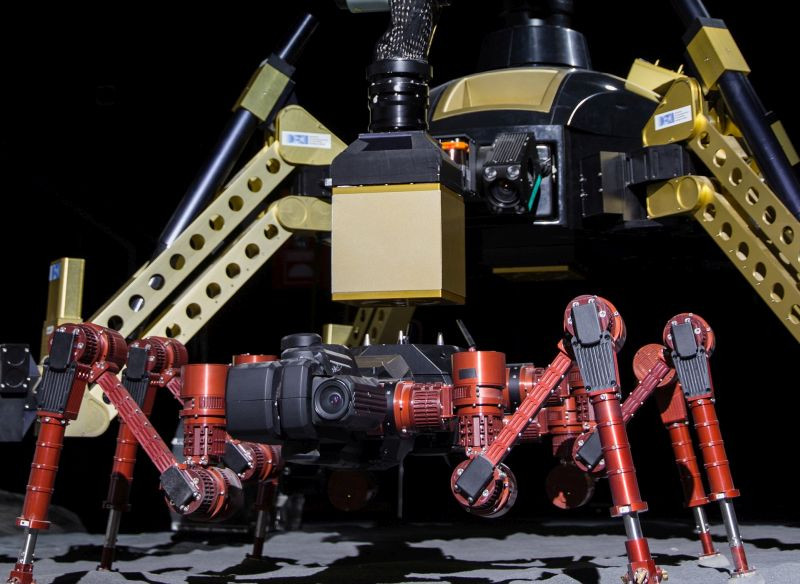
\includegraphics[width=0.8\linewidth]{pictures/RIMRES-final-14}\\
  %\vspace{-2ex}
  \caption[A sample image]
          {A sample image. This is a longer caption than that used for the index.}
  \label{fig:RIMRES-final-14}
  %\vspace{-3ex}
\end{figure}

\begin{figure}%[b]
\vspace{-2ex}
	\centering
    %% setup sizes
    \setlength{\subfigureWidth}{0.32\textwidth}
    \setlength{\graphicsHeight}{33mm}
    %% kill hyper-link highlighting
    \hypersetup{hidelinks=true}%
    %% the figures
	\begin{subfigure}[t]{\subfigureWidth}
        \centering
		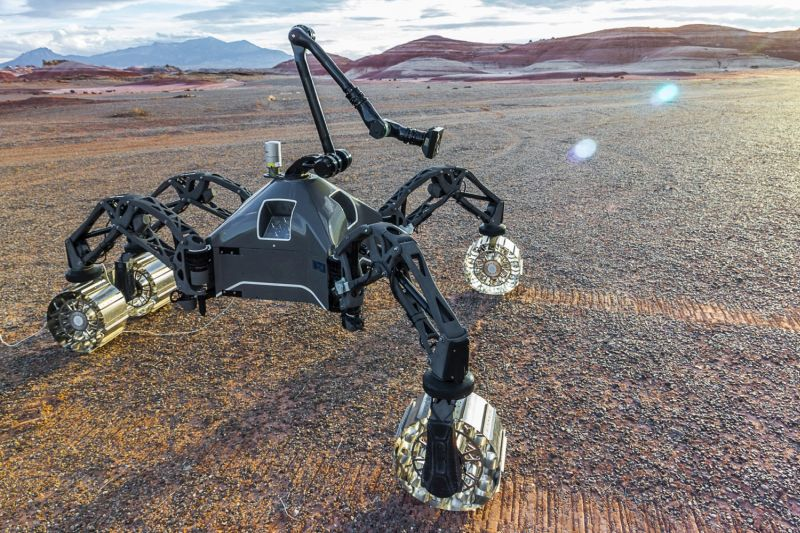
\includegraphics[height=\graphicsHeight]{pictures/SherpaTT_QuasiTripod}
		\subcaption{Quasi tripod pose}
		\label{fig:SherpaTT_QuasiTripod}
	\end{subfigure}\hfill
	\begin{subfigure}[t]{\subfigureWidth}
        \centering
		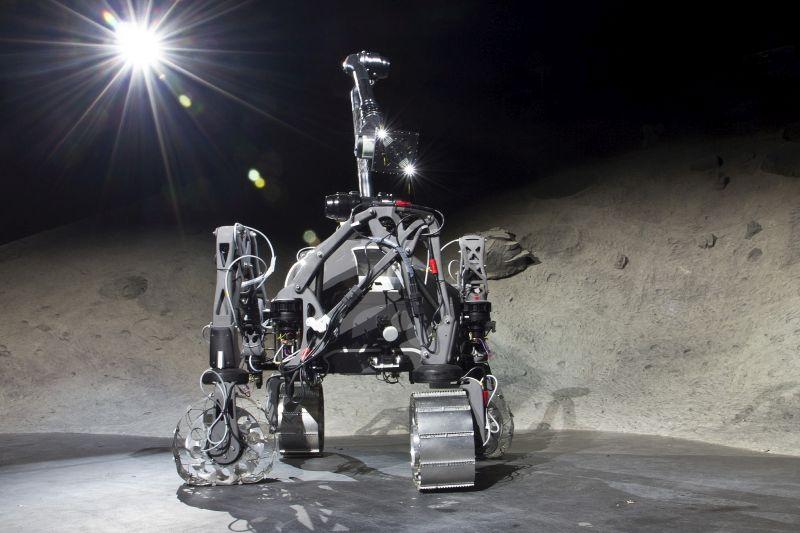
\includegraphics[height=\graphicsHeight]{pictures/SherpaTT_Stow}
		\subcaption{Compact stow pose of legs}
		\label{fig:SherpaTT_Stow}
	\end{subfigure}\hfill
    \begin{subfigure}[t]{\subfigureWidth}
        \centering
		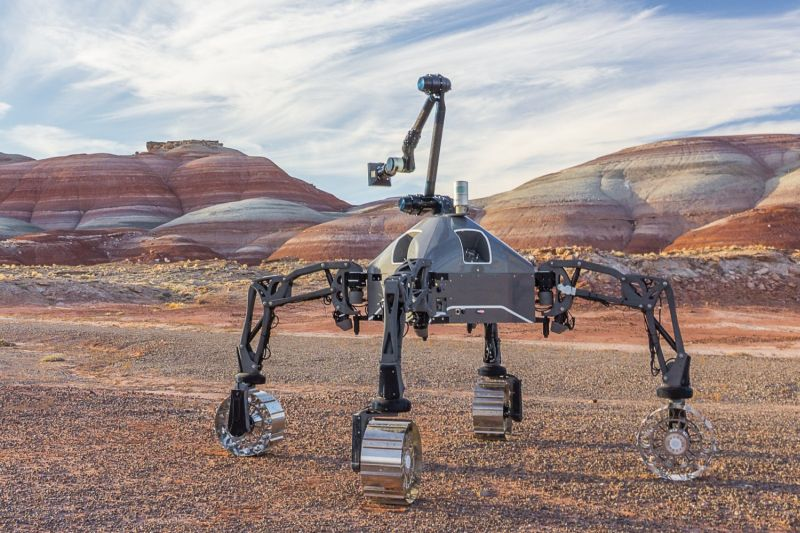
\includegraphics[height=\graphicsHeight]{pictures/SherpaTT_HighPose}
		\subcaption{High body pose in CrossStance}
		\label{fig:SherpaTT_HighPose}
	\end{subfigure}\\[0.8ex]
%% 2nd row
    \begin{subfigure}[t]{\subfigureWidth}
        \centering
		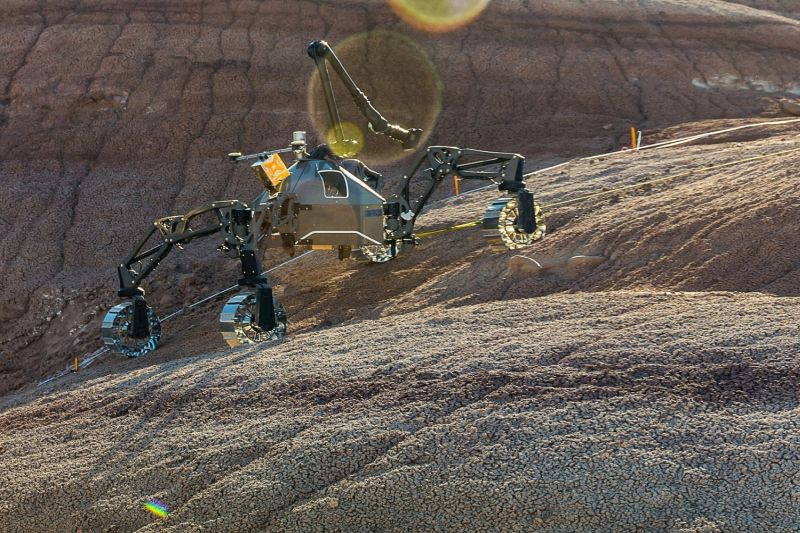
\includegraphics[height=\graphicsHeight]{pictures/SherpaTT_RPA_Utah}
		\subcaption{Body roll-pitch control in sloping natural terrain}
		\label{fig:SherpaTT_RPA_Utah}
	\end{subfigure}\hfill
	\begin{subfigure}[t]{\subfigureWidth}
        \centering
		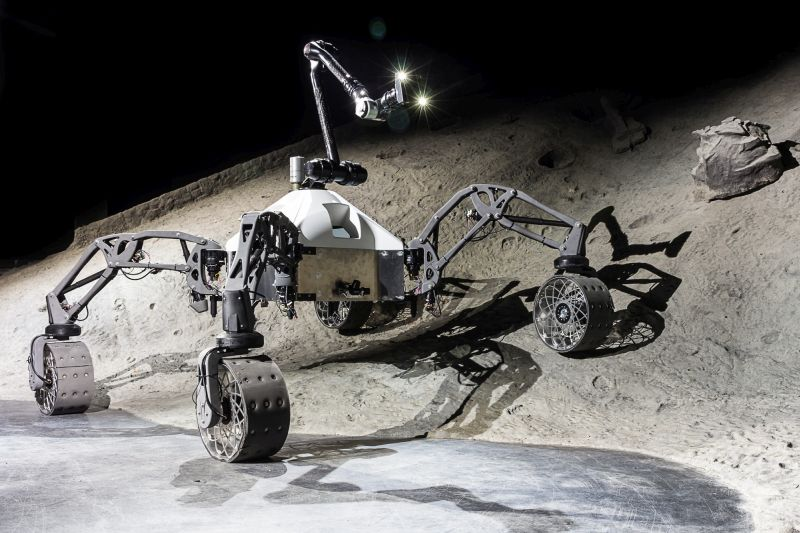
\includegraphics[height=\graphicsHeight]{pictures/SherpaTT_RPA_Crater}
		\subcaption{Body roll-pitch control in artificial crater}
		\label{fig:SherpaTT_RPA_Crater}
	\end{subfigure}\hfill
    \begin{subfigure}[t]{\subfigureWidth}
        \centering
		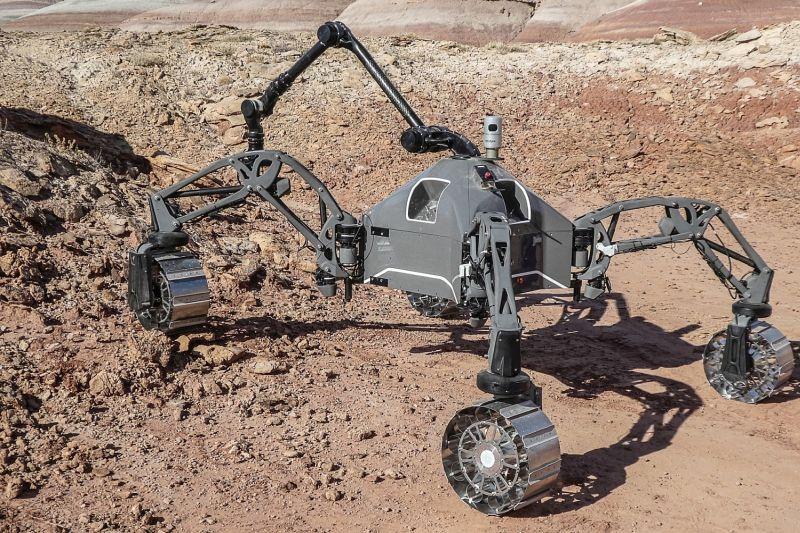
\includegraphics[height=\graphicsHeight]{pictures/SherpaTT_SamplingUtah}
		\subcaption{Approaching a sampling spot in natural terrain}
		\label{fig:SherpaTT_SamplingUtah}
	\end{subfigure}
	\caption{Example of a figure with subfigures}
	\label{fig:SherpaTT}
\vspace{-2ex}
\end{figure}


\begin{table}%[h]
%\vspace{-2ex}
  %\centering
  \hypersetup{hidelinks=true}
  %
  \caption[Exemplary table]{Exemplary table.
  \dissExtraCaption{With an example of an extra caption. Should be used with optional caption.}
  }
  \label{tab:Design:ComparisonSherpaSherpaTT}
  \begin{footnotesize}
      \begin{tabular}{l| rrr r ll r rr}
        \toprule
         \rowcolor{tableheadingcolor}
        System  & Leg length & Mass    & Mass & \ac{DoF}         & vert. & horz. & min stow  & \multicolumn{2}{c}{compactness}\\
        \rowcolor{tableheadingcolor}
                & zero pose &  (leg)  & total  & (leg)   & stroke &  stroke &volume    & footprint & volume \\
        \midrule
        \cellcolor{tablesubheadingcolor}Sherpa      & 976\unitmm & 25\unitkg & 160\unitkg &6          & 900\unitmm
%        \color{captionTextColor}{$^{\ast}$}
        & 260\unitmm
%        \color{captionTextColor}{$^{\ast\ast}$}
        &  2.24\unitcubmeter & 0.40 & 0.64\\
        \cellcolor{tablesubheadingcolor}SherpaTT\hspace{-1mm}    & 977\unitmm & 26\unitkg & \massSherpaTT &5          & 775\unitmm & 485\unitmm & 1.67\unitcubmeter & 0.79 & 0.72\\
        \bottomrule
      \end{tabular}
  \end{footnotesize}
\end{table}





\section{Structure of Thesis}
The structure of this thesis is illustrated in \refFig{fig:structure_diagram}. \todo{if you do not want to use citations, check \swCmd{styles/structureGraphFunctions.tex} with the example of an alternative \swCmd{\textbackslash drawChapterBox} command}
From the publications forming this cumulative thesis, those related to each chapter are provided in the respective box.
Further publications of the author are cited at the appropriate places in each paragraph.



\begin{figure}%[htb]
    \begin{center}
        %%%%%%%%%%%%%%%%%%%%%%%%%%%%%%%%%%%%%%%%
%%% structural graph of thesis document
%%%%%%%%%%%%%%%%%%%%%%%%%%%%%%%%%%%%%%%%


%% helper for minipages
%%  \begin{minipage}[outerPos][height][innerPos]{width}
%%	     Beispieltext
%%  \end{minipage}
%% outerPos (optional; c,t,b): where the minipage is on the page (center, top, bottom)
%% height (optional): height o minipage, regardless of contents
%% innerPos (optional; c,t,b): where the content is (center, top, bottom)

% set some dimension variables for minipages
\newlength{\structureGraphHeight}
\setlength{\structureGraphHeight}{100mm}

\newlength{\chapterboxWith}
\setlength{\chapterboxWith}{0.45\linewidth}

\newlength{\chapterboxHeight}
\setlength{\chapterboxHeight}{21mm}





%%% the actual graph







%%%%%%%%%%%%%%%%%%%%%%%%%%%%%%%%%%%%%%%%%%%%%%%%%%%%%%%%%%%%%%%%%%%%%%%%%%%%%%%%%%%%%%%%%%%%%%%%%%%%%%%%%%%%%
%% this is the actual structure plot
%% settings are in   thesis_colors.sty   and   styles/structrueGraphFunctions.tex
%%



%\begin{tcolorbox}[code={\pgfkeysalsofrom{\outerboxoptions}},
%                  title=Thesis: \newline\qq{\myWorkingTitle}]
    %external raster
    \begin{tcbraster}[ code={\pgfkeysalsofrom{\outerrasteroptions}} ]
            %ROW 1                                                        % |-- SINGLE-box-Options
            \partbox{Intro}{}{                                            % v
                \begin{tcboxedraster}[ code={\pgfkeysalsofrom{\innerrastersinglecoloptions}} ]{blankest}
                        \rule{0.25\linewidth}{0pt}% remove for dual
                        \drawChapterbox{sec:introduction}{\introCites}%
                        %\rule{0.2\linewidth}{0pt}%
                \end{tcboxedraster}
            }
            % ROW2
            \partbox{Foundations}{}{
                \begin{tcboxedraster}[ code={\pgfkeysalsofrom{\innerrasterdualcoloptions}} ]{blankest} 
                        \drawChapterboxSota{sec:sota}{ \sotaCites }%
                        \drawChapterbox{sec:ReqirementsConditions}{ ~ }%
                \end{tcboxedraster}
            }
            % ROW3                                                       % |-- DUAL-box-Options
            \partbox{Design}{}{                                          % v
                \begin{tcboxedraster}[ code={\pgfkeysalsofrom{\innerrasterdualcoloptions}} ]{blankest} %<- no drawn box or white space around inner boxes
                        \drawChapterbox{sec:RobotDesign}{ \designCites }%
                        \drawChapterbox{sec:control}{ \controlCites }%
                \end{tcboxedraster}
            }
            %ROW 4
            \partbox{~~Experi-}{mentation}{
                \begin{tcboxedraster}[ code={\pgfkeysalsofrom{\innerrastersinglecoloptions}} ]{blankest}
                        \rule{0.25\linewidth}{0pt}%
                        \drawChapterbox{sec:Experiments}{ \expCites }%
                        %\rule{0.2\linewidth}{0pt}%
                \end{tcboxedraster}
            }
            %ROW 5
            \partbox{Conclusion}{}{
                \begin{tcboxedraster}[ code={\pgfkeysalsofrom{\innerrastersinglecoloptions}} ]{blankest}
                        \rule{0.25\linewidth}{0pt}%
                        \drawChapterbox{sec:ConclusionOutlook}{ \conclusionCites }%
                        %\rule{0.2\linewidth}{0pt}%
                \end{tcboxedraster}
           }
            %ROW 6
            \partbox{Appendix}{}{
                \begin{tcboxedraster}[ code={\pgfkeysalsofrom{\innerrastertriplecoloptions}} ]{blankest}
                        %\rule{0.25\linewidth}{0pt}%
                        \drawAppendixbox{sec:Appendix:AdditionalMaterial}{ ~ }%
                        \drawAppendixbox{sec:Appendix:MoreStuff}{ ~ }%
                        \drawAppendixbox{sec:Appendix:Enough}{ ~ }%
                        %\rule{0.2\linewidth}{0pt}%
                \end{tcboxedraster}
            }
    \end{tcbraster}
%\end{tcolorbox}	














    \end{center}
    \vspace{-1ex}
    \caption{Structure of this thesis and related publications per chapter.}
    \label{fig:structure_diagram}
    %\vspace{-1.8ex}
\end{figure}


\section{Bibliography Remarks}
\label{sec:intro:BibRemarks}
\todo{run the \swCmd{make\_bib.bat} file or the command lines within to generate the bibliography}
To better distinguish between the author's own publications and citations from literature, different citation marks are applied:
\begin{compactitem}
  \item Citations from the author's own publications are plain numbered, \eg~\citeown{myPubA}, \citeown{myPubB}. 
  \item Citations from literature are using the author-year format, \eg~\citesota{Wilcox2012}.
\end{compactitem}




%%%%%%%%%%%%%%%%%%%%%%%%%%%%%%%%%%%%%%%%%%%%%%%%%%%%%%%




%%%%%%%%%%%%%%%%%%%%%%%%%%%%%%%%%%%%%%%%%%%%%%%%%%%%%%%
\chapter{State of the Art}
\label{sec:sota}
%\acresetall                 %% reset all acronym abbreviations and write first appearance long
%\acused{CAD}
\acused{DoF}
\acused{EEPROM}
\acused{FPGA}
\acused{GPS}
\acused{HD}
\acused{LED} %%define ackronyms that are "common sense"

\shinyChapterQuote{A shiny quote for the start?}
       {If you like to.}

This chapter gives a brief overview on the \SOTA of the main topics of this thesis.
\todo[inline]{adapt to your own thesis!}

%\chapterSupportedBy{\sotaCites}
%\sotaCites
%\todo{check long list vs. short list macros!}
\chapterSupportedBy{\sotaCitesLong}




\section{A Section of this Chapter}
\label{sec:sota:ASection}
%\input{sections/.tex}

\section{Another Section of this Chapter}
\label{sec:sota:AnotherSection}
%\input{sections/.tex}

%%%%%%%%%%%%%%%%%%%%%%%%%%%%%%%%%%%%%%%%%%%%%%%%%%%%%%%


%%%%%%%%%%%%%%%%%%%%%%%%%%%%%%%%%%%%%%%%%%%%%%%%%%%%%%%
\chapter{The Martian Environment}
\shinyChapterQuote{Maybe I’ll post a consumer review. “Brought product to surface of Mars. It stopped working. 0/10.”}
  {Andy Weir, The Martian.}
\label{sec:MartianEnvironment}
%\acresetall                 %% reset all acronym abbreviations and write first appearance long
%\acused{CAD}
\acused{DoF}
\acused{EEPROM}
\acused{FPGA}
\acused{GPS}
\acused{HD}
\acused{LED} %%define ackronyms that are "common sense"
%\input{sections/martian-environment/references.tex}



\section{Dust}
\label{sec:MartianEnvironment:Dust}
%\input{sections/s.tex}

% Martian Season - start with images
% Regolith, dust, and craters, other elements
% Settle with locations DTMS

Great dust storms (area > 10e6 km2) occur with a yearly probability of 30\% to 80\%. \citepower{Kerslake1999}

Local dust storms (area < 10e6 km2) occur with a 5\% probability in Mars equatorial regions and have only a minor impact on seasonal insulation due to their limited size, duration (a few days), and moderate OD (~1). \citepower{Kerslake1999}

the dust accumulation rate is assumed to be 5\% of that measured by Pathfinder \citepower{Kerslake1999}

Losses from lander vehicle shadowing and terrain masking are not yet modeled pending better definitions of lander configuration and landing sites. \citepower{Kerslake1999}

For desirable near-equatorial landing sites (not in canyons), shadowing and terrain masking losses will be small. This is due to high sun angles (that create short shadows) and the large component of diffuse solar insolation near dusk and dawn (when the terrain masking effect is largest). \citepower{Kerslake1999}


\section{Dust Storms}
\label{sec:MartianEnvironment:DustStorms}
%\input{sections/s.tex}

%%%%%%%%%%%%%%%%%%%%%%%%%%%%%%%%%%%%%%%%%%%%%%%%%%%%%%%


%%%%%%%%%%%%%%%%%%%%%%%%%%%%%%%%%%%%%%%%%%%%%%%%%%%%%%
\chapter[Requirements and Design Drivers: Heterogeneous Modular Multi-Robot Systems] %%for toc
        [Design Drivers: Heterogeneous Modular Multi-Robot Systems] %% for head
        {Requirements and Design Drivers: Heterogeneous Modular \\ Multi-Robot Systems} %%for chapter page
\label{sec:ReqirementsConditions}
\shinyChapterQuote{A shiny quote for the start?}
       {If you like to.}
This is an example chapter for usage of three types of chapter headings. (see source file)
%\acresetall                 %% reset all acronym abbreviations and write first appearance long
%\acused{CAD}
\acused{DoF}
\acused{EEPROM}
\acused{FPGA}
\acused{GPS}
\acused{HD}
\acused{LED} %%define ackronyms that are "common sense"

%%%%%%%%%%%%%%%%%%%%%%%%%%%%%%%%%%%%%%%%%%%%%%%%%%%%%%



%%%%%%%%%%%%%%%%%%%%%%%%%%%%%%%%%%%%%%%%%%%%%%%%%%%%%%
\chapter{\ElecMech Rover Design}
\label{sec:RobotDesign}
%\acresetall                 %% reset all acronym abbreviations and write first appearance long
%\acused{CAD}
\acused{DoF}
\acused{EEPROM}
\acused{FPGA}
\acused{GPS}
\acused{HD}
\acused{LED} %%define ackronyms that are "common sense"

%%-----------------------------------------------
\shinyChapterQuote{[...] development of robotic mechanization and control architectures that enable roving into
adverse, challenging terrain -- areas that can change dramatically over short distances -- is of considerable importance.}
{\citesota{Schenker2001}}


%%-----------------------------------------------
This chapter ... \todo{what is to be expected of this chapter?}

%%-----------------------------------------------
%\chapterSupportedBy{\designCites}
%\designCites
%\todo{check long list vs. short list macros!}
\chapterSupportedBy{\designCitesLong}



%%-----------------------------------------------

\section{Design Considerations}
\label{sec:design:considerations}
\lipsum


\section{System Design: Mechanics}
\label{sec:design:mechanics}
\input{sections/RobotDesign_mechanics.tex}


\section{Summary and Conclusion}
\label{sec:design:SummaryConclusion}
\todo[inline]{Always a good idea to give a short conclusion per chapter}



%%%%%%%%%%%%%%%%%%%%%%%%%%%%%%%%%%%%%%%%%%%%%%%%%%%%%%



%%%%%%%%%%%%%%%%%%%%%%%%%%%%%%%%%%%%%%%%%%%%%%%%%%%%%%
\chapter{Control System Design}
\label{sec:control}
%\acresetall                 %% reset all acronym abbreviations and write first appearance long
%\acused{CAD}
\acused{DoF}
\acused{EEPROM}
\acused{FPGA}
\acused{GPS}
\acused{HD}
\acused{LED} %%define ackronyms that are "common sense"
%%-----------------------------------------------
\shinyChapterQuote{If everything seems under control, \newline
       you're just not going fast enough.}
       {Mario Andretti}
%%-----------------------------------------------

This chapter \todo{...shows what?}

%%-----------------------------------------------
%\chapterSupportedBy{\mcsCites}
%\mcsCites
%\todo{check long list vs. short list macros!}
\chapterSupportedBy{\controlCitesLong}

%%-----------------------------------------------




%\begin{itemize}
%%   \setlength\itemsep{0em}
%%   \setlength\topsep{0em}
%  \item reactive control and advantages for planetary rovers, p2/14
%  \item layers of control... HL, MW, LL
%  \item
%\end{itemize}


\section{A}
\label{sec:control:Structure}
%\input{sections/ControlSystemDesign_.tex}
\lipsum


\section{Coordinate Systems for Locomotion Control}
\label{sec:control:kinematicsConsiderations}
%\input{sections/ControlSystemDesign_.tex}


\section{Summary and Conclusion}
\label{sec:control:Conclusion}
This chapter presents ....

\lipsum






%%%%%%%%%%%%%%%%%%%%%%%%%%%%%%%%%%%%%%%%%%%%%%%%%%%%%%



%%%%%%%%%%%%%%%%%%%%%%%%%%%%%%%%%%%%%%%%%%%%%%%%%%%%%%
\chapter{Experimental Evaluation}
\label{sec:Experiments}
%\acresetall                 %% reset all acronym abbreviations and write first appearance long
%\acused{CAD}
\acused{DoF}
\acused{EEPROM}
\acused{FPGA}
\acused{GPS}
\acused{HD}
\acused{LED} %%define ackronyms that are "common sense"
%%-----------------------------------------------
\shinyChapterQuote{No amount of experimentation can ever prove me right; \newline
       a single experiment can prove me wrong.}
       {Albert Einstein}


%%-----------------------------------------------


This chapter of the thesis summarizes the experiments and results conducted for ... \todo{!}


%%-----------------------------------------------
%\chapterSupportedBy{\expCites}
%\expCites
%\todo{check long list vs. short list macros!}
\chapterSupportedBy{\expCitesLong}

%%-----------------------------------------------

\section{General Experimental Setup and Evaluation Methods}
\label{sec:Experimente:Setup}
%\input{sections/experiments_setup.tex}


\section{Experiment 1}
\label{sec:Experiments:Exp1}
%\input{sections/experiments_1.tex}

\section{Experiment 2}
\label{sec:Experiments:Exp2}
%\input{sections/experiments_2.tex}


\section{Summary and Conclusion} 
\label{sec:Experiments:Conclusion}
This chapter presents the \electromech system design of the two rover versions Sherpa and SherpaTT.
General design decisions valid for both systems are presented with the main influences resulting from the respective \ac{MRS}.
Apart from the kinematic design of the suspension systems, the central power management is discussed as this is a central part for the rovers to be a fully functional subsystem of a modular \ac{MRS}.

A manipulation arm for both rovers is developed using an evolutionary algorithm for morphology optimization.
Several use-cases are defined and a trajectory for the arm is built to test the use-cases in a physical simulation for fitness evaluation of the respective individuum.
The arm is then manufactured following a biologically inspired manufacturing methodology.
%Both rover systems make use of the same manipulation arm.

Comparing the main features of both implemented rover systems shows basically the same leg length of the first and second suspension generation, \refTab{tab:Design:ComparisonSherpaSherpaTT}.
The mass per leg as well as the total system mass are nearly identical as well.
With five \ac{DoF} per leg, the second generation suspension has one \ac{DoF} less per leg.
Horizontal and vertical \ac{LEP} movements in Sherpa are coupled, while they are independent in SherpaTT.
Note that the vertical and horizontal stroke listed for SherpaTT in the table are those resulting from the currently set software-joint limits as also shown in \refFig{fig:SherpaTT_Workspace-2d}.
Exploiting the full mechanical range as provided in \refTab{tab:AntriebsdatenSherpaTT} results in 860\unitmm vertical and 629\unitmm horizontal stroke.

\begin{table}[h]
%\vspace{-2ex}
  %\centering
  \hypersetup{hidelinks=true}
  %
  \caption[Comparison of main features of suspension system generations and rovers]{Comparison of main features of suspension system generations and rovers.
  %\dissExtraCaption{The stow footprint is measured using the \acp{LEP}, while the stow volume is a cuboid enclosing all parts of the rover, including those overhanging the \ac{LEP}'s footprint.}
  }
  \label{tab:Design:ComparisonSherpaSherpaTT}
  \begin{footnotesize}
      \begin{tabular}{l| rrr r ll r rr}
        \toprule
         \rowcolor{tableheadingcolor}
        System  & Leg length & Mass    & Mass & \ac{DoF}         & vert. & horz. & min stow  & \multicolumn{2}{c}{compactness}\\
        \rowcolor{tableheadingcolor}
                & zero pose &  (leg)  & total  & (leg)   & stroke &  stroke &volume    & footprint & volume \\
        \midrule
        \cellcolor{tablesubheadingcolor}Sherpa      & 976\unitmm & 25\unitkg & 160\unitkg &6          & 900\unitmm
%        \color{captionTextColor}{$^{\ast}$}
        & 260\unitmm
%        \color{captionTextColor}{$^{\ast\ast}$}
        &  2.24\unitcubmeter & 0.40 & 0.64\\
        \cellcolor{tablesubheadingcolor}SherpaTT\hspace{-1mm}    & 977\unitmm & 26\unitkg & \massSherpaTT &5          & 775\unitmm & 485\unitmm & 1.67\unitcubmeter & 0.79 & 0.72\\
        \bottomrule
      \end{tabular}
  \end{footnotesize}
  %\begin{scriptsize}
       % \vspace{-2mm}
%        \begin{flushleft}
%            \color{captionTextColor}{
%                $^{\ast}$ ~~~only possible with simultaneously changing horizontal position
%            \newline
%                $^{\ast\ast}$ ~\,only possible with simultaneously changing vertical position
%            %\newline
%%                $^{\ast\ast\ast}$ software safety limitation of IL and OL actuators, full range with mechanical limits: 860\unitmm and 629\unitmm see \refTab{tab:AntriebsdatenSherpaTT}.
%            }
%    \end{flushleft}
%    \end{scriptsize}
    %\vspace{-3ex}
\end{table}

Due to improved arrangement of the \ac{DoF}, the minimum stow volume is reduced from 2.24\unitcubmeter to 1.67\unitcubmeter.
This is also reflected in the values of compactness provided in the table; these values are based on the isoperimetric quotient:
The ratio of the area of the footprint to the area of a circle with the same perimeter is built.
A circle is the most compact shape in two-dimensional space,
therefore, the ratio ranges between 0 and 1 with high compactness being close to 1.
Similarly the compactness of the three-dimensional envelope volume is calculated using a sphere as most compact volume.
In both cases, the new design achieves higher compactness values.
%Higher compactness bears the potential for better fitting into a lander structure for transfer to Moon or Mars.



Apart from the compactness, the new arrangement of the \ac{DoF} allows to place the \ac{LEP} in a three-dimensional workspace compared to a two-dimensional spherical surface.
This design generates internal mobilities, that can be used to facilitate deployment and pickup of immobile elements in the \ac{MRS}.
Furthermore, the position and orientation of the central body in the support polygon can be changed without moving the wheels over the ground, which is beneficial for \ac{CoG} relocations in intricate slopes with low traction surface material.

A six \ac{DoF} \ac{FTS} is present in each leg of the new suspension system design.
Direct ground contact force measurement becomes available with this sensor, which in turn allows improved load balancing between the rover's ground contact points.

To conclude, with basically the same dimensioning (size, weight), superior properties are presented with the second suspension system design.
The subsequent chapters focus on the control and evaluation of this new suspension system and the rover SherpaTT.





%%%%%%%%%%%%%%%%%%%%%%%%%%%%%%%%%%%%%%%%%%%%%%%%%%%%%%



%%%%%%%%%%%%%%%%%%%%%%%%%%%%%%%%%%%%%%%%%%%%%%%%%%%%%%
\chapter{Conclusion and Outlook}
\label{sec:ConclusionOutlook}
\todo[inline]{The very important findings of this thesis go here}
%%%%%%%%%%%%%%%%%%%%%%%%%%%%%%%%%%%%%%%%%%%%%%%%%%%%%%


%% redefine headers for Bibliography
\makeevenhead{ruled}{\itshape\leftmark}{}{}
\makeoddhead{ruled}{}{}{\itshape\rightmark}
\pagestyle{ruled}

\addTocCaption{Bibliography}

\begin{small}
%\addcontentsline{toc}{chapter}{Bibliography}
%\bibliographystyle{alpha}
%\bibliography{../../ownPublications} % literaturverzeichnis
\bibliographysota{sections/sota}
\bibliographyown{sections/ownPublications} %%liegt über root-verzeichnis der eigentlichen Diss...
\bibliographymarsenv{references/marsenv}
\bibliographymoonenv{references/moonenv}
\bibliographypower{references/power}
\end{small}
\cleardoublepage


\todo[inline]{check printing/digital flag for link colors}


%% redefine headers for Appendix
\makeevenhead{ruled}{\scshape Appendix \leftmark}{}{}
\makeoddhead{ruled}{}{}{\itshape\rightmark}
\pagestyle{ruled}

\begin{appendix}
\addTocCaption{Appendix}
%\addcontentsline{toc}{chapter}{Appendix}
%\backmatter %%changes formatting!

\chapter{Additional Material}
\label{sec:Appendix:AdditionalMaterial}
This chapter contains additional material such as system specifications and experiment data previously not published in this form.
All data presented here is based on the publications \AppACites.


\section{first}
lorem ipsum
%\clearpage

\section{second}
\lipsum 
%\clearpage





%\addcontentsline{toc}{chapter}{Accumulated Publications}
\chapter{More Stuff}
\label{sec:Appendix:MoreStuff}


%% this is how to teak the toc:
%% add extra spacing to get caption on next page of toc
%\cftaddtitleline{toc}{chapter}{\vspace{5mm}}{} %extra neg. space in toc

\chapter{Enough!}
\label{sec:Appendix:Enough}

\end{appendix}



\end{document}
